% \title{ Сравнение подходов обучения на базе словаря и MAP к проблеме повышения разрешения на примере изображений автомобильных номеров }
\title{Повышение разрешения изображений автомобильных номеров}
\author{
  \begin{tabular}[4cm]{rl}
 Автор:                & Улитин А.~А., 591 гр. \\
 Научный руководитель: & к.\,ф.-м.\,н., доцент~Вахитов А.~Т. \\
 % Рецензент: & инженер-программист Пименов А. А. \\
 \end{tabular}
 \vspace{3em} \\
 Санкт-Петербургский государственный университет \\
 Факультет прикладной математики -- процессов управления \\
 Кафедра моделирования электромеханических и компьютерных систем \\
 }
\date{Санкт-Петербург, 2013 год}

\begin{frame}{}
		\maketitle
\end{frame}

\section{Задача}
\begin{frame}{Задача Super-resolution}
  Задача Super resolution --- качественно повысить разрешения изображения.
  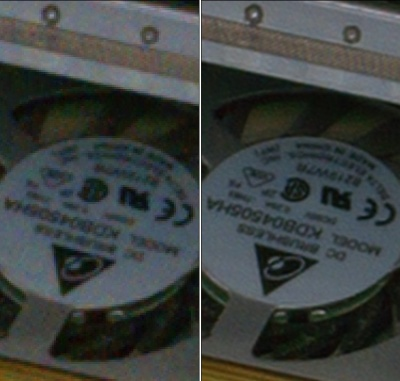
\includegraphics[height=\textheight]{content/An_example_of_super_resolution_with_still_RAW_photo.jpg}
\end{frame}

\begin{frame}{Почему это возможно}
  Для повышения разрешения используется дополнительная информация
  \begin{itemize}
    \item Знание параметров съемки (размытие, движение камеры~и~т.п.)
    \item Знание о типе снимаемого объекта (текст, лица, и т.п.)
    \item Использование нескольких изображений, снятых с разных ракурсов
  \end{itemize}
  которая влияет на конечное изображение

  Применимость:
  \begin{itemize}
    \item Препроцессинг для других алгоритмов компьютерного зрения
    \item Извлечение дополнительной информации с нескольких снимков для получения одного кадра с высоким разрешением
  \end{itemize}
\end{frame}

\begin{frame}{PSNR}

  $$ \mathrm{MSE}(\tilde{x},x) = \frac{1}{m\,n}\sum_{i=0}^{m-1}\sum_{j=0}^{n-1} [\tilde{x}(i,j) - x(i,j)]^2$$

  И обозначим величину обратную ей и выраженную на логарифмической шкале как $\mathrm{PSNR}(\tilde{x},x)$.
  $$ \mathrm{PSNR}(\tilde{x},x) &= 10 \cdot \log_{10} \left( \frac{\mathrm{MAX}_I^2}{\mathrm{MSE}(\tilde{x},x)} \right)
  $$
Где $MAX_I$ максимально возможное значение яркости изображения
\end{frame}

\section{Подход FastSR}
\begin{frame}{Подход FastSR}
  \begin{itemize}
    \item Superresolution of License Plates in Real Traffic Videos \\
      (K. V. Suresh, G. Mahesh Kumar, and A. N. Rajagopalan) \\
      Основная идея -- использование шаговой оптимизации с адаптивным регуляризатором.
      \begin{itemize}
        \item Для восстановление использует последовательную оптимизацию с
          регуляризаторами
        \item Использует несколько изображений
      \end{itemize}
  \end{itemize}
\end{frame}
\begin{frame}{Постановка задачи}
 $$y_r = D H_R W_R x + n_r,~ ~ ~ 1 \leq r \leq m$$
 где:
 \begin{itemize}
   \item $x$ оригинальное изображение
   \item $y_r$ наблюдение r
   \item $D$ матрица понижение разрешения
   \item $W$ матрица геометрического искажения
   \item $H_R$ матрица размытия наблюдения r
   \item $n_r$ шум наблюдения r
   \item $m$ количество наблюдений
 \end{itemize}
 %Задача найти
 %$$ \tilde{x} = \underset{\hat{x}}{\operatorname{argmax}}~  PSNR(\hat{x},x)$$
 Задача обозначить границы применимости метода FastSR, исследование требования к изображениям для получения наилучшего
 значения PSNR (очевидно, в модели)
\end{frame}


\begin{frame}{Проделанная работа с июля 2013 }
  \begin{itemize}
    \item Проверена гипотеза о связи G (корректирующая функция) с ошибкой ME
    \item Получены raw изображения автомобильных номеров для проверки алгоритма в реальных условиях. Т.к. мы не знаем
      истинное изображение, то получить численную оценку невозможно. Разница в возможности прочтения не обнаружена.
    \item Рефакторинг
  \end{itemize}
\end{frame}

\section{Планы}
\begin{frame}{Планы}
  Совместно со студентов Матмеха пишем генератор автомобильных номеров. Возможно, что перебор и подсчет MSE даст лучший
  результат, чем обобщенный алгоритм FastSR.
\end{frame}

\section{Список литературы}
\begin{frame}[allowframebreaks]{Список литературы}
\nocite{suresh2007superresolution}
\nocite{tian2011survey}
\nocite{gonzalez2002woods}
\bibliographystyle{plain}
\bibliography{bib}
\end{frame}
